% Schelling focal point example (Potts): nine figures, select the same one
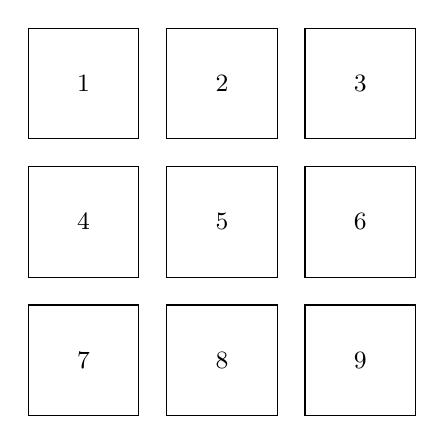
\begin{tikzpicture}[x=1pt, y=1pt, every node/.style={inner sep=1pt, font=\small}]
  \draw (0,0) rectangle (40,40);
  \draw (50,0) rectangle (90,40);
  \draw (100,0) rectangle (140,40);
  \draw (0,50) rectangle (40,90);
  \draw (50,50) rectangle (90,90);
  \draw (100,50) rectangle (140,90);
  \draw (0,100) rectangle (40,140);
  \draw (50,100) rectangle (90,140);
  \draw (100,100) rectangle (140,140);
  \node[anchor=south] at (20,116) {1};
  \node[anchor=south] at (70,116) {2};
  \node[anchor=south] at (120,116) {3};
  \node[anchor=south] at (20,66) {4};
  \node[anchor=south] at (70,66) {5};
  \node[anchor=south] at (120,66) {6};
  \node[anchor=south] at (20,16) {7};
  \node[anchor=south] at (70,16) {8};
  \node[anchor=south] at (120,16) {9};
\end{tikzpicture}
